%!TEX root = ../bdr.tex
\chapter{Основні приклади користування {\TeX}}

В розділі подаються в ілюстративній формі основні принципи створення текстових дукоментів засобами комп'ютерної
типографії {\LaTeX}. Поданої інформації має вистачити для того, щоб почати створювати спеціалізовані текстові 
документи маючи мінімальній досвід роботи з такою системою. 

\section{Текст}
А це просто текст...

Порожній рядок означає, що це був абзац

\textbf{Lorem Ipsum is simply dummyl}  text of the printing and typesetting industry. Lorem Ipsum has been the industry's standard dummy text ever since the 1500s, when an unknown printer took a galley of type and scrambled it to make a type specimen book. 

It has survived not only five centuries, but also the leap into electronic typesetting, remaining essentially unchanged. It was popularised in the 1960s with the release of Letraset sheets containing Lorem Ipsum passages, and more recently with desktop publishing software like Aldus PageMaker including versions of Lorem Ipsum. 

%\lipsum[1-2]
\section{Списки}
Маркований список:
\begin{itemize}
\item Зелений;
\item Жовтий;
\item Білий.
\end{itemize}

Нумерований дворівневий список:
\begin{enumerate}
\item Колір
      \begin{enumerate}
      \item Зелений;
      \item Жовтий;
      \item Білий.
      \end{enumerate}	
\item Температура
      \begin{enumerate}
      \item Теплий;
      \item Холодний.
      \end{enumerate}
\end{enumerate}
 

\section{Рисунки}

Вставка рисунків робиться дуже просто:

\begin{figure}[h]
\caption{Опис рисунку}
\end{figure}

Далі можна вставити і сам рисунок (рис. \ref{fig:tux}). Він має бути у графічному файлі ({*}.jpg, {*}.png тощо). 

\begin{figure}[h]
 \centering
\includegraphics{img/Tux.png}
 \caption{Пінгвін}
 \label{fig:tux}
\end{figure}

%\begin{figure}[h]
% \centering\includegraphics[width=0.25\textwidth]{example-image-a}
% \caption{Назва рисунку}
% \label{image:label}
%\end{figure}

Рисунок можна винести і в додаток (додаток \ref{apdx:text}), \label{linkpage} а посилання на нього залишити в основній частині роботи (рис. \ref{apdxfig:tux}).
Можна вручную вставляти картинки і прописувати кожний параметр.
Параметр width визначає ширину рисунку. У цьому прикладі вона дорівнюватиме ширині текста \verb|\textwidth|. Замість \verb|\textwidth| можна вказати значення від 0.1 до 1. \verb|\label| потрібна для того, щоби потім можна було послатись на цю картинку, як тут.

\begin{figure}[!htb]
 \centering
 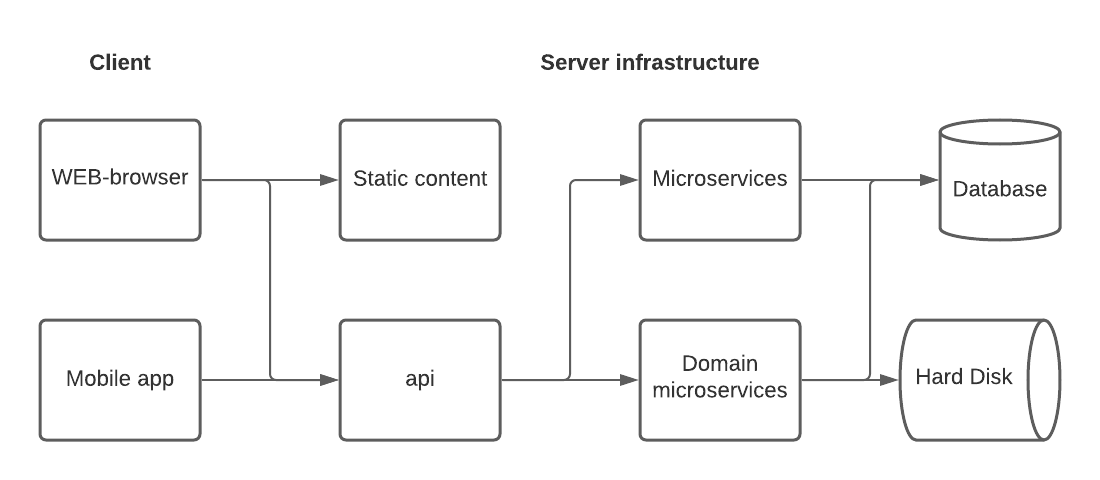
\includegraphics[width=0.8\textwidth]{img/fig1.png}
 \caption{Назва рисунку}
 \label{fig:fig1}
\end{figure}

\section{Таблиці}
Таблиці  - це складний об'єкт. Тому всі параметри треба прописувати вручну

\begin{table}[h!]
\centering
\begin{tabular}{|c|c|c|c|} 
 \hline
 Стопець1 & Стопець2 & Стопець3 & Стопець4 \\ [0.5ex] 
 \hline
 \multirow{3}{5em}{Декілька рядків} & 6 & 87837 & 787 \\ 
  &  7 & 78 & 5415 \\
   & 545 & 778 & 7507 \\
   & 545 & 18744 & 7560 \\
   & 88 & 788 & 6344 \\ [1ex] 
 \hline
\end{tabular}
\caption{Приклад роботи з таблицею}
\label{table:1}
\end{table}

%\begin{table}[h]
%	\caption{\label{table:2}Функціональна залежність параметрів ...}
	%\label{table:2}
%	\begin{tabular}{|c|c|c|}
%		\hline 
%		Індекс & Показник 1 & Показник 2\tabularnewline
%		\hline 
%		\hline 
%		1 & 2 & 3\tabularnewline
%		\hline 
%		4 & 5 & 6\tabularnewline
%		\hline 
%	\end{tabular}
%\end{table}

\begin{table}[h]
\caption{\label{table:label}Назва таблиці}
\hspace{\floatindent}   %place table with indentation 
\begin{tabular}{|c|c|c|}
\hline 
Індекс & Показник 1 & Показник 2 \\
\hline\hline 
1 & 2 & 3 \\
\hline 
4 & 5 & 6 \\
\hline 
\end{tabular}
\end{table}

Для табл. \ref{table:label} вже можете побачити легенду, яка на відміну від рисунків розташована зверху.

Великі таблиці можна повертати на 90 градусів:

%\begin{sidewaystable}
%	\centering{}
%	\caption{Набір компонентів.}
%	\begin{tabular}{|c|>{\raggedright}p{0.25\columnwidth}|>{\centering}p{0.15\columnwidth}|>{\centering}p{0.1\columnwidth}|}
%	\hline 
%	№ & Компонент  & Маса & К-сть\tabularnewline
%	\hline 
%	\hline 
%	1 & Компонент А & 12.8 & 100\tabularnewline
%	\hline 
%	2 & Компонент Б & 7.88 & 12\tabularnewline
%	\hline 
%	3 & Компонент В & 83.89 & 44\tabularnewline
%	\hline 
%	\end{tabular}
%\end{sidewaystable}

Більше про таблиці можна прочитати \href{https://www.overleaf.com/learn/latex/Tables}{тут}.

\clearpage{}

\section{Формули...}
Для вставки формул можна користуватись конструювати формули будь-якої складності. Ось приклад формули із нумерацією:

\begin{equation}
	\text{f=}\sqrt[12]{\sum\left(\beta*\xi\right)*\frac{z}{\arctan(123)}}*\top f(z)
\end{equation}

А це ще одна нумерована формула

\begin{equation}
	\varpi=\cos\text{q}\sqrt{{x}{y}}
\end{equation}

Формули з нумерацією    
\begin{equation}
    f(x)=\frac{x}{1+x^2}
\end{equation}

Ще одна формула    
\begin{equation}
    x^n + y^n = z^n
\end{equation}
    
А так прописуються формули, де нумерація не потрібна \(x^2 + y^2 = z^2\).

Другий спосіб - це вставити формулу між символам долара: $x^2 + y^2 = z^2$. 

Пояснення до змісту формул робиться так:

\begin{equation}
T = 2\pi\sqrt{\frac{m}{k}}, 
\end{equation}

\begin{explanation}
\fitem $k$ -- коефіцієнт жорсткості пружини; 
\item $m$ -- маса тягарця.
\end{explanation}

                  
З одиницею вимірювання в квадратних дужках,

\begin{equation}
\label{eq:explan}
I = \frac{U}{R}~[A]
\end{equation}

або в круглих дужках,

$$I = \frac{220}{100}~(\text{А}).$$

Перенесення формул робиться математичними знаками, повторюючи цей знак на початку наступного рядка. При знакові множення «$\cdot$» його замінюють знаком «$\times$».

\begin{align}
\label{xt:eq}
y(t) &= \frac{1}{{\rho}\,{S}\,{C_{f}}\,\sin\alpha}\Big(\ln\Big(\frac{1}{1962\,m}\Big(10\,v_0\sqrt{\rho\,S\,C_f\,\sin^3\alpha}\,\times \nonumber\\  &\times\cos\Big(\frac{3\,t\,\sqrt{218\,\rho\,S\,C_f\,\sin\alpha}}{20\,\sqrt{m}}\Big)\Big)^2\Big)\,m\Big).
\end{align}

Читайте \href{https://www.overleaf.com/learn/latex/Operators}{тут} про математичні оператори.

\section{Межі}
    
    Межа \(\lim_{x\to\infty} f(x)\) всередені тексту.
    І між рядками:
    \[
    \lim_{x\to\infty} f(x)
    \]
Про суми і ліміти читайте 
\href{https://www.overleaf.com/learn/latex/Integrals,_sums_and_limits#Sums_and_products}{тут}.

\section{Символи}
$\alpha A$ - грецькі,  $ \lambda; \Lambda$ - физичні величины=и, $\exists; \forall$ - логічні символм\\
За \href{https://www.overleaf.com/learn/latex/List_of_Greek_letters_and_math_symbols}{цим посиланням} можна одержати інформацію про інші символи. 

\section{Зноски, примітки та інш.}
У тексті зручно робити різноманітні зноски та примітки. Для цього їх достатньо встановити у необхідному місці, а форматування зробить свою потужну роботу. Ось приклад зноски, що розташується знизу \footnote{Це тест до зноски 1}. 

\section{{\LaTeX} Wiki}
Повне введення у {\LaTeX} читайти \href{https://www.texlive.info/CTAN/info/lshort/russian/lshortru.pdf}{тут}.

Про інтеграли інструкції 
\href{https://www.overleaf.com/learn/latex/Integrals,_sums_and_limits#Integrals}{тут}.



